\documentclass[a4paper]{article}
\usepackage[T2A]{fontenc}
\usepackage[utf8]{inputenc}
\usepackage[ukrainian]{babel}
\usepackage{tikz}
\usepackage{lastpage} 
\usepackage[left=2.5cm, right=1.5cm, top=1.5cm, bottom=2.7cm]{geometry}
\usepackage{fancyhdr}
\usepackage{amsmath, amssymb, amstext} % Математичні символи
\usepackage{fp}
\usepackage{ragged2e}

\usepackage{listings}

\usepackage{xifthen} % Для умовних перевірок

% \usepackage{fontspec}
% \setmainfont{Times New Roman}

\usepackage{caption}


% \usepackage{graphicx}

\pagestyle{fancy}
\fancyhf{}
\renewcommand{\headrulewidth}{0pt}
\renewcommand{\footrulewidth}{0pt}

% \pagestyle{empty}

\newcommand{\makrosCalc}[1]{
    \FPeval{\the\fpresult}{#1}
}

\newcommand{\makrosmytitle}[2]{
    \thispagestyle{empty}
    \centering
    \textbf{Міністерство освіти і науки України}\\
    \textbf{КИЇВСЬКИЙ ПОЛІТЕХНІЧНИЙ УНІВЕРССИТЕТ}\\[2cm]
    \raggedleft
    Кафедра автоматизації та систем неруйнівного контролю\\
    Група ПМ-11
    \vfill
    \centering
    \textbf{ПРОЕКТУВАННЯ СИСТЕМ АВТОМАТИЗАЦІЇ}\\[1cm]
    \textbf{ЗВІТ З #1}\\[1cm]
    \textbf{\huge #2}
    \vfill
    \begin{flushleft}
        Керівник  \qquad\qquad\quad \hfill\qquad (підпис)\hfill 
        д.т.н., проф. Черепанська І. Ю.\\
        \hfill (дата)\\[2cm]
        Виконавець\hfill (підпис)\hfill Осипчук О. Г.\\
        \hfill (дата)
    \end{flushleft}
    \vfill
    \centering
    2025
}

\newcommand{\makrosFrameBig}[2]{
    \thispagestyle{empty} % Вимикає номер сторінки на першій сторінці
    
    \begin{tikzpicture}[remember picture, overlay]
        \begin{scope}[shift={([xshift = 20 mm, yshift = 10 mm]current page.south west)}]
            \draw[line width=2] (0,0) rectangle (180 mm,277 mm);
        \end{scope}
    \end{tikzpicture}
    
    \begin{tikzpicture}[remember picture, overlay]
        \begin{scope}[shift={([xshift = 20 mm, yshift = 10 mm]current page.south west)}, x=1mm, y=1mm]
            \draw[line width=2] (0,0) rectangle (180,40);
            \draw[line width=2]  (7,40) -- (7, 25);
            \draw[line width=2] (17,40) -- (17, 0);
            \draw[line width=2] (40,40) -- (40, 0);
            \draw[line width=2] (55,40) -- (55, 0);
            \draw[line width=2] (65,40) -- (65, 0);
            \draw[line width=2] (135,25) -- (135,0);
            \draw[line width=2] (140,15) -- (140,20);
            \draw[line width=2] (145,15) -- (145,20);
            \draw[line width=2] (150,25) -- (150,15);
            \draw[line width=2] (165,25) -- (165,15);
        
            \draw (0,35) -- (65, 35);
            \draw[line width=2] (0,30) -- (65, 30);
            \draw[line width=2] (0,25) -- (180, 25);
            \draw (0,20) -- (65, 20);
            \draw (0,15) -- (65, 15);
            \draw (0,10) -- (65, 10);
            \draw (0,5) -- (65, 5);
        
            \draw[line width=2] (135,20) -- (180, 20);
            \draw[line width=2] (135,15) -- (180, 15);
            
            \node at (3.5, 27.5) {Зм.};
            \node at (12, 27.5) {Лист};
            \node at (28.5, 27.5) {№ докум.};
            \node at (47.5, 27.5) {Підпис};
            \node at (60, 27.5) {Дата};
            
            \node at (7, 22.5) {Розроб.};
            \node at (6.5, 17.5) {Перев.};
            \node at (8.5, 7.5) {Н. Контр.};
            \node[align=left] at (5, 2.5) {Затв.};
            
            \node at (142.5, 22.5) {Літ.};
            \node at (157.5, 22.5) {Аркуш};
            \node at (172, 22.5) {Аркушів};
        
            \node[align=left, font=\itshape, anchor=south west, scale=0.9] at (16, 20) {Погорєлов Б.Ю.};
            \node[align=left, font=\itshape, anchor=south west, scale=0.8] at (16, 15) {Черепанська І.Ю.};
            \node[align=left, font=\itshape, anchor=south west, scale=0.8] at (16, 0) {Черепанська І.Ю.};
        
            \node[anchor=center, font=\itshape, scale=1.5] at (122, 32) {#1};
            \node[align=center, font=\itshape, anchor=center] at (100, 12) {#2};
            \node[align=left, font=\itshape, anchor=south west, scale=0.9] at (135, 5) {КПІ ім. І. Сікорського, ПБФ};
            \node[anchor=center, font=\itshape] at (158, 17) {2};
            \node[anchor=center, font=\itshape] at (172, 17) {\pageref{LastPage}};    
        \end{scope} 
    \end{tikzpicture}
}

\newcommand{\makrosFrameSmall}[1]{
    % \thispagestyle{empty} % Вимикає номер сторінки на першій сторінці
    
    \begin{tikzpicture}[remember picture, overlay]
        \begin{scope}[shift={([xshift = 20 mm, yshift = 10 mm]current page.south west)}]
            \draw[line width=2] (0,0) rectangle (180 mm,277 mm);
        \end{scope}
    \end{tikzpicture}
    
    \begin{tikzpicture}[remember picture, overlay]
        \begin{scope}[shift={([xshift = 20 mm, yshift = 10 mm]current page.south west)}, x=1mm, y=1mm]
            \draw[line width=2] (0,0) rectangle (180,15);
            \draw[line width=2] (7,0) -- (7, 15);
            \draw[line width=2] (17,0) rectangle (43,15);
            \draw[line width=2] (55,0) rectangle (64,15);
            \draw[line width=2] (170,0) -- (170, 15);

            \draw[line width=2] (0,5) -- (64, 5);
            \draw               (0,10) -- (64, 10);
            \draw[line width=2] (170,8) -- (180, 8);

            \node[anchor=center, scale=0.8] at (3.5, 2.5) {Змн.};
            \node[anchor=center, scale=0.9] at (12, 2.5) {Арк.};
            \node[anchor=center] at (30, 2.5) {№~докум.};
            \node[anchor=center, scale=0.9] at (49, 2.5) {Підпис};
            \node[anchor=center, scale=0.9] at (59, 2.5) {Дата};
            \node[anchor=center, font=\itshape, scale=1.5] at (115, 7.5) 
                {#1};
            \node[anchor=center] at (175, 12) {Арк.};
            \node[anchor=center] at (175, 4) {\thepage};
            
        \end{scope}
    \end{tikzpicture}
}

% % \makrosLab{1}{Шифр}{Назва}
% \newcommand{\makrosLab}[3]{ 
%     \fancyfoot[C]{\makrosFrameSmall{#2}}
%     \ifthenelse{\equal{#2}{л}}%    
%     % \makrosmytitle{#1}{#3}
%     \newpage
%     \makrosFrameBig{#2}{#3}
%     \justify
%     \fontsize{14}{16}\selectfont
%     \section*{Лабораторна робота №#1}
% }

% Оголошуємо змінні
\newcommand{\mytitlegenitive}{}
\newcommand{\mytitle}{}
\newcommand{\shyfr}{}

% \makrosLab{номер}{п чи л}{Назва}
\newcommand{\makrosLab}[3]{ 


    % Перевіряємо другий аргумент
    \ifthenelse{\equal{#2}{л}}%
        {
            \renewcommand{\mytitle}{Лабораторна робота №#1}
            \renewcommand{\mytitlegenitive}{ЛАБОРАТОРНОЇ РОБОТИ №#1}
            \renewcommand{\shyfr}{ПМ1108.04.00.0#1 ЛР}
        }%
        { \ifthenelse{\equal{#2}{п}}%
            {
                \renewcommand{\mytitle}{Практична робота №#1}
                \renewcommand{\mytitlegenitive}{ПРАКТИЧНОЇ РОБОТИ №#1}
                \renewcommand{\shyfr}{ПМ1108.04.00.0#1 ПР}
            }%
            {\section*{ПОМИЛКА}}%
        }%

    % Використання змінних
    \fancyfoot[C]{\makrosFrameSmall{\shyfr}}
    \makrosmytitle{\mytitlegenitive}{#3}
    \newpage
    \makrosFrameBig{\shyfr}{#3}
    \justifying
    \vspace*{-20mm}
    \fontsize{14}{16}\selectfont
    \section*{\mytitle}
}


\usepackage{amsmath, amssymb}
\usepackage{graphicx}
\usepackage{float}
\usepackage{caption}
\usepackage{siunitx}

\begin{document}
    \makrosLab{2}{л}{
        Розробка та складання схем \\
        електричних принципових керування \\ 
        промисловими двигунами
    }

    \section*{Тема роботи}
    Розробка та складання схем електричних принципових керування
    промисловими двигунами

    \section*{Мета роботи}
    Вивчити будову та принцип дії промислових двигунів
    різних типів, як складових систем автоматичного
    керування / регулювання / контролю. Навчитися складати схеми електричні
    принципові для керування промисловими двигунами різних типів.

    \section*{Вихідні дані (Варіант 09)}
Для варіанту 9:
\begin{itemize}
    \item Номінальна потужність на валу, \( P_{\text{ном.мех}} = 100 \, \text{кВт} \)
    \item Коефіцієнт потужності, \( \cos \varphi_{\text{ном}} = 0.95 \)
    \item Номінальна швидкість обертання, \( n_{\text{ном}} = 2950 \, \text{об/хв} \)
    \item Коефіцієнт перенавантажної здатності, \( \gamma = 2.25 \)
    \item ККД, \( \eta = 89\% \)
    \item Коефіцієнт кратності пускового струму, \( \alpha =  5.5\)
    \item Коефіцієнт кратності пускового моменту, \( \beta = 2.4 \)
\end{itemize}

    \newpage
    
    \section*{Завдання}
Трифазний асинхронний двигун з короткозамкненим ротором має такі параметри:
\begin{enumerate}
    \item напруга живлення: $380/220$ В;
    \item номінальна потужність на валу: $P_{\text{ном.мех}}$;
    \item номінальна швидкість: $n_{\text{ном}}$;
    \item коефіцієнт корисної дії: $\eta$;
    \item коефіцієнт потужності: $\cos \varphi_{\text{ном}}$;
    \item коефіцієнт кратності пускового струму: $\alpha$;
    \item коефіцієнт кратності пускового моменту: $\beta = \frac{M_{\text{пуск}}}{M_{\text{н}}}$;
    \item коефіцієнт перенавантажної здатності: $\gamma = \frac{M_{\text{max}}}{M_{\text{н}}}$.
\end{enumerate}

Двигун увімкнено за схемою "зірка" до мережі з лінійною напругою $U_{\text{лін}} = 380$ В, частотою $f = 50$ Гц.

З врахуванням даних визначити:
\begin{enumerate}
    \item споживану потужність: активну, реактивну, повну;
    \item споживаний струм;
    \item пусковий струм;
    \item ємність конденсаторів для підвищення $\cos\varphi$ до $0,95$ при вмиканні їх за схемами "зірка" та "трикутник", побудувати векторні діаграми напруги і струмів та трикутник потужностей;
    \item обертаючі моменти двигуна: номінальний, пусковий, критичний;
    \item номінальне і критичне значення ковзання;
    \item обертаючий момент двигуна при значеннях ковзання: $S = 0$; $S_{\text{ном}}$; $0,8S_{\text{кр}}$; $S_{\text{кр}}$; $1,2S_{\text{кр}}$; $0,2$; $0,4$; $0,6$; $0,8$; $1$.
\end{enumerate}
    
    \newpage 
    \section*{Схеми}

\begin{figure}[h]
    \centering
    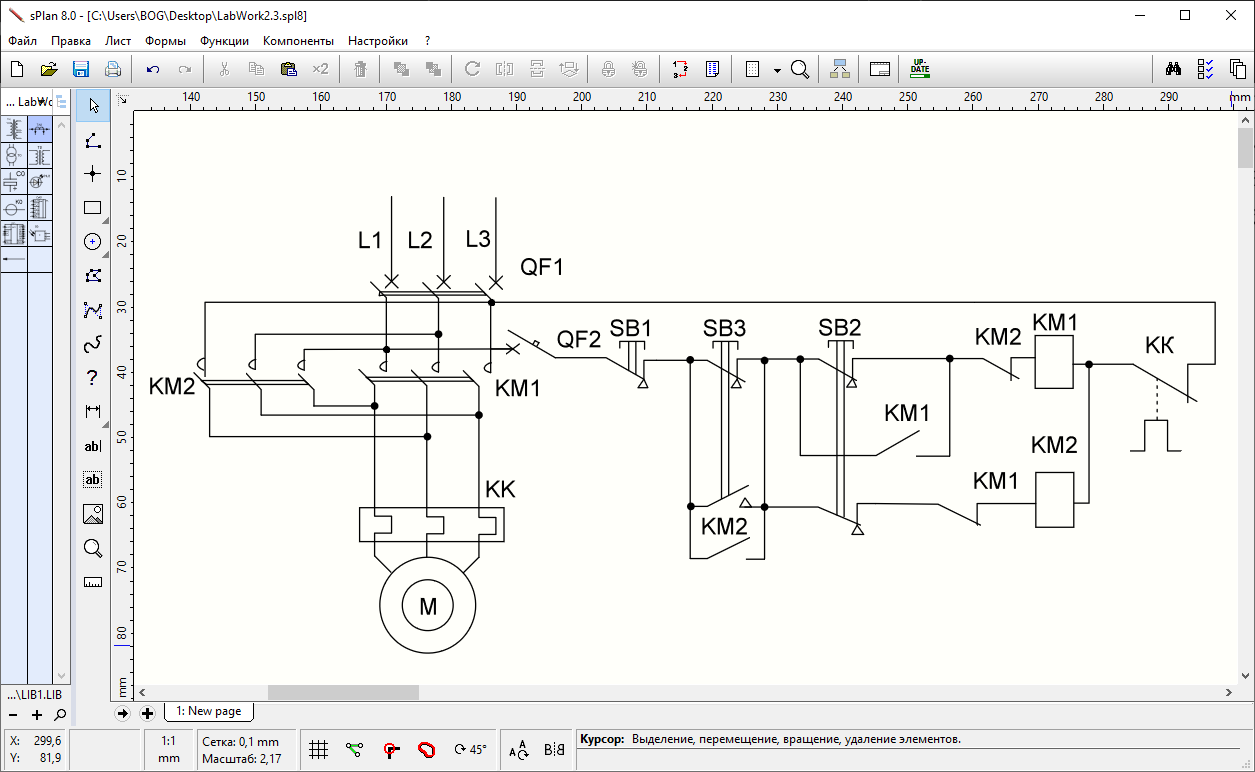
\includegraphics[width=0.45\textwidth]{imgs/LW2.1.png}
    \caption*{Рис. 2.1: Схема електрична принципова реверсивного керування асинхронним електродвигуном}
\end{figure} 

\begin{figure}[h]
    \centering
    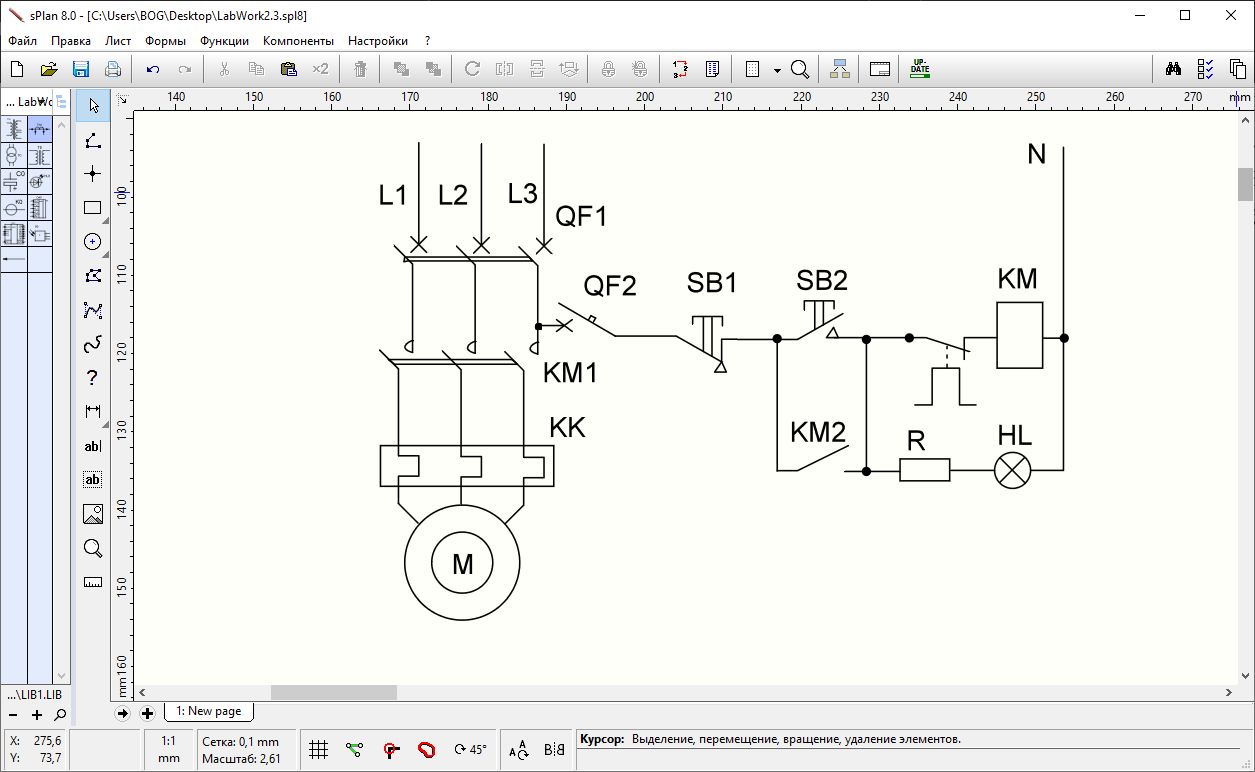
\includegraphics[width=0.45\textwidth]{imgs/LW2.2.png}
    \caption*{Рис. 2.2: Схема електрична принципова нереверсивного керування асинхронним електродвигуном}
\end{figure} 

\begin{figure}[h]
    \centering
    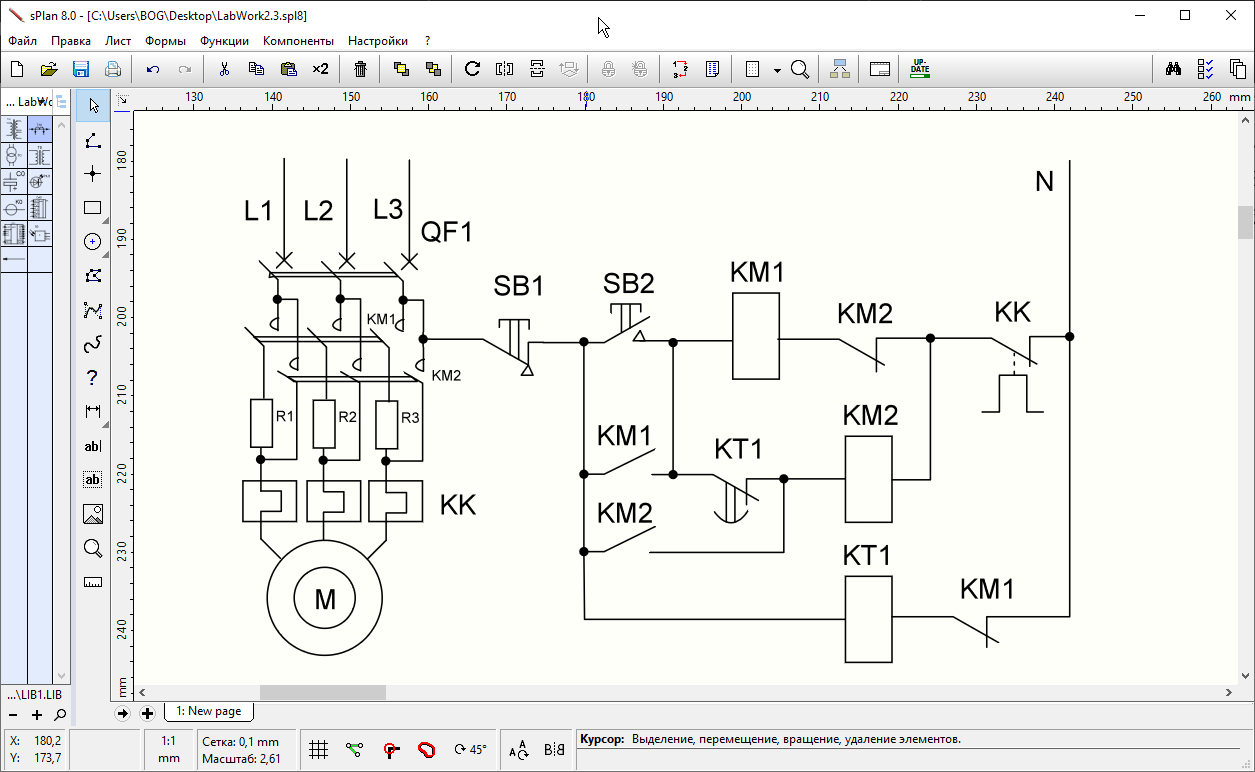
\includegraphics[width=0.5\textwidth]{imgs/LW2.3.png}
    \caption*{Рис. 2.3: Схема електрична принципова керування трифазним асинхронним електродвигуном з короткозамкненим ротором з обмеженням  пускового струму і моменту активними опорами}
\end{figure} 

\begin{figure}[h]
    \centering
    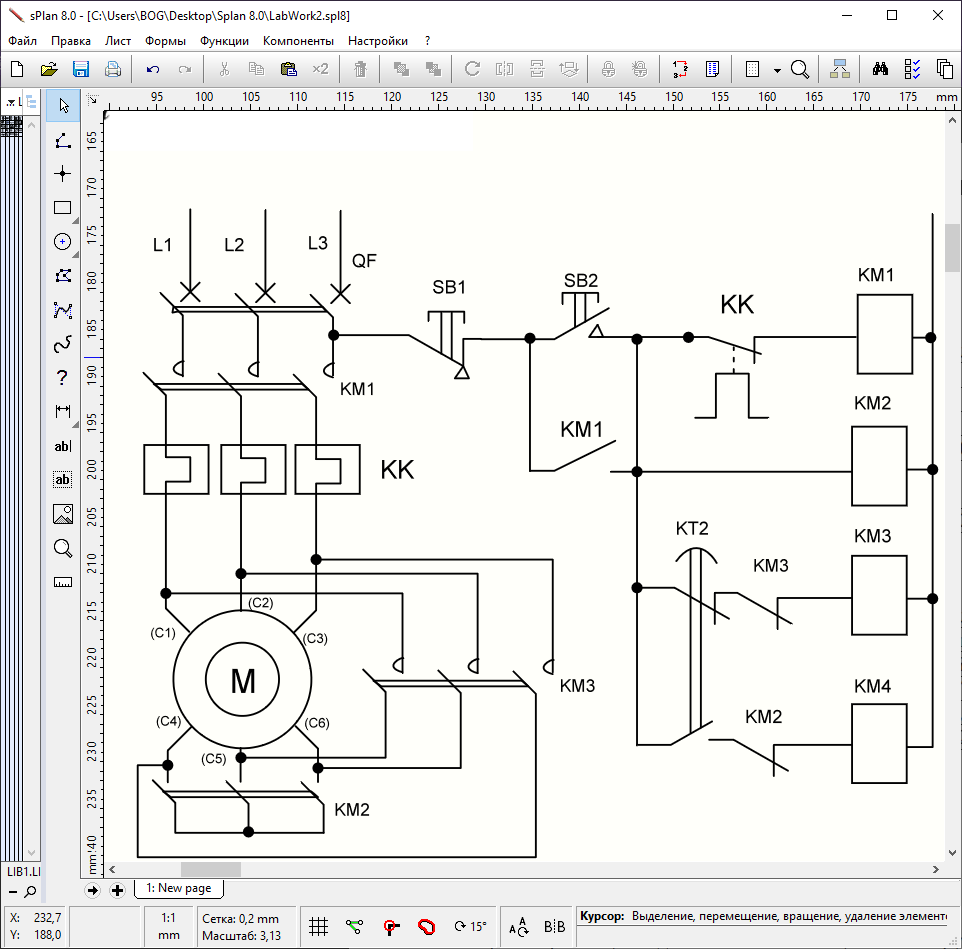
\includegraphics[width=0.45\textwidth]{imgs/LW2.4.png}
    \caption*{Рис. 2.4: Схема електрична принципова керування трифазним асинхронним електродвигуном з перемиканням обмотки статора iз «зірки» на «трикутник» при пуску}
\end{figure}

\begin{figure}[h]
    \centering
    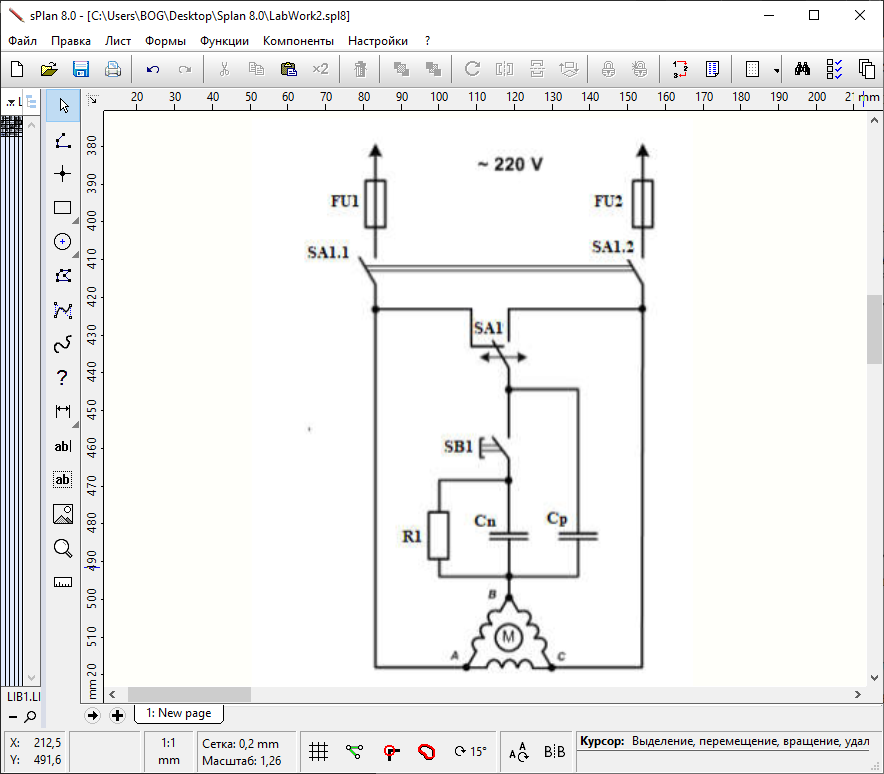
\includegraphics[width=0.5\textwidth]{imgs/LW2.4.2.png}
    \caption*{Рис. 2.5: Схема електрична принципова}
\end{figure}

\newpage


\section*{Розрахунок споживаної потужності}
\begin{align*}
P_1 &= \frac{P_{\text{ном.мех}}}{\eta} = \frac{100\,\text{кВт}}{0.89} \approx 112.36\,\text{кВт} \\
S &= \frac{P_1}{\cos \varphi} = \frac{112.36}{0.95} \approx 118.27\,\text{кВА} \\
Q &= \sqrt{S^2 - P_1^2} = \sqrt{118.27^2 - 112.36^2} \approx 38.99\,\text{квар}
\end{align*}

\section*{Розрахунок струмів}
\begin{itemize}
    \item Фазна напруга (схема "зірка"): $U_{\text{ф}} = \frac{U_{\text{лін}}}{\sqrt{3}} \approx 219.39\ \text{В}$
\end{itemize}
\begin{align*}
I_1 &= \frac{S \cdot 10^3}{\sqrt{3} \cdot U_{\text{лін}}} = \frac{118270}{\sqrt{3} \cdot 380} \approx 179.8\ \text{А} \\
I_{\text{пуск}} &= \alpha \cdot I_1 = 5.5 \cdot 179.8 \approx 989.1\ \text{А}
\end{align*}

\section*{Розрахунок моментів}
\begin{align*}
M_{\text{ном}} &= \frac{9550 \cdot P_{\text{ном.мех}}}{n_{\text{ном}}} = \frac{9550 \cdot 100}{2950} \approx 323.73\ \text{Нм} \\
M_{\text{пуск}} &= \beta \cdot M_{\text{ном}} = 2.4 \cdot 323.73 \approx 776.95\ \text{Нм} \\
M_{\text{max}} &= \gamma \cdot M_{\text{ном}} = 2.25 \cdot 323.73 \approx 728.39\ \text{Нм}
\end{align*}

\section*{Ковзання}

Пара полюсів (2 полюси): $p = 1$
\begin{align*}
n_1 &= \frac{60 \cdot f}{p} = 60 \cdot 50 = 3000\ \text{об/хв} \\
s_{\text{ном}} &= \frac{n_1 - n_{\text{ном}}}{n_1} = \frac{3000 - 2950}{3000} = 0.0167
\end{align*}

\section*{Розрахунок ємності конденсаторів для компенсації реактивної потужності}

\begin{align*}
Q &= 38.99\ \text{квар} = 38990\ \text{вар} \\
C_{\text{зв}} &= \frac{Q}{3 \cdot \omega \cdot U_{\text{ф}}^2},\quad \omega = 2\pi f = 314.16\,\text{рад/с} \\
C_{\text{зв}} &= \frac{38990}{3 \cdot 314.16 \cdot 219.39^2} \approx 8.52\,\mu\text{Ф} \\
C_{\text{тр}} &= 3 \cdot C_{\text{зв}} \approx 25.56\,\mu\text{Ф}
\end{align*}

\section*{Залежність моменту від ковзання}

\begin{table}[H]
\centering
\caption*{Рис. 2.7: Таблиця залежності моменту від ковзання}
\begin{tabular}{|c|c|}
\hline
\textbf{Ковзання $s$} & \textbf{Момент $M(s)$, Нм} \\
\hline
0.0000 & 0.00 \\
0.0167 & 236.68 \\
0.0800 & 710.62 \\
0.1000 & 728.39 \\
0.1200 & 716.45 \\
0.2000 & 582.71 \\
0.4000 & 342.77 \\
0.6000 & 236.23 \\
0.8000 & 179.30 \\
1.0000 & 144.24 \\
\hline
\end{tabular}
\end{table}

\begin{figure}[h]
    \centering
    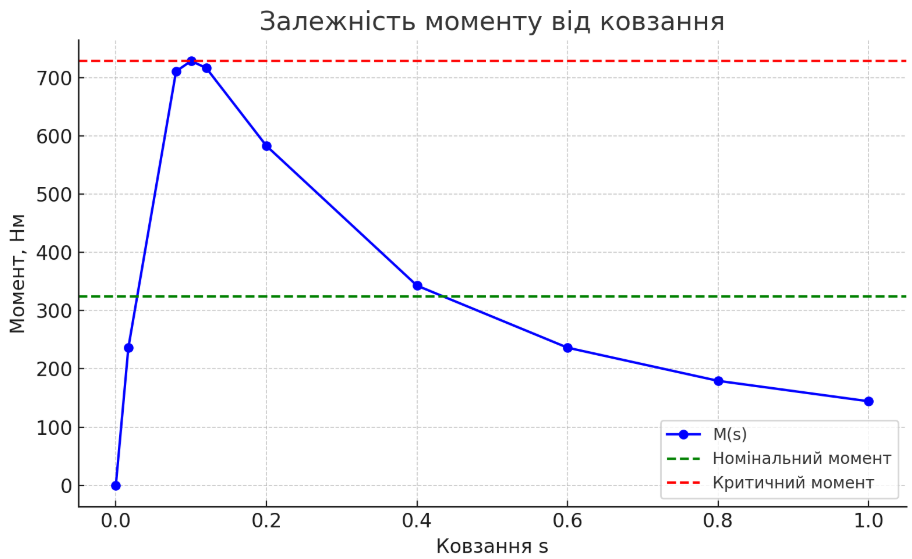
\includegraphics[width=0.7\textwidth]{imgs/LW2_moment_vs_slip.png}
    \caption*{Рис. 2.7: Графік залежності моменту двигуна від ковзання}
\end{figure}

\section*{Висновки}

Отримані результати дозволяють оцінити параметри роботи трифазного асинхронного двигуна, його енергетичні характеристики та вибір необхідних ємностей для підвищення коефіцієнта потужності.

\section*{Контрольні питання}
\begin{enumerate}
    \item Чому асинхронний двигун так називається? \\
    Асинхронний двигун називається так тому, що частота обертання його ротора не співпадає з частотою обертання магнітного поля статора (яка визначається частотою змінного струму). Різниця між цими частотами називається ковзанням.
    
    \item Чому є небажаною велика сила пускового струму? \\
    Велика сила пускового струму небажана, оскільки вона може призвести до значних механічних та електричних навантажень на двигун і мережу, викликати пошкодження ізоляції проводів, зменшити термін служби обладнання, а також викликати перевантаження трансформаторів і підстанцій.
    
    \item Що використовують для зниження сили пускового струму? \\
    Для зниження сили пускового струму використовують спеціальні пристрої, такі як стартери з обмеженням струму, трансформатори з регульованим напругою або пристрої плавного пуску, що забезпечують поступове збільшення напруги на двигуні.
\end{enumerate}


\end{document}